\chapter{Using Copulas for Joining Credal Sets}\label{chap:joining_credal_sets}
In the presence of multiple sources of uncertainty, the question of how to join those sources arises. Using probability distributions, the usual method for joining probability distributions is to use copulas (section \ref{sec:copulas}). However, there are multiple ways of joining imprecise models using a copula. Sections \ref{sec:robust_method} , \ref{sec:joint_mass} and \ref{sec:aggregation_method} present three different ways of joining credal sets using a copula. Those three methods are not equivalent, we thus explore their similarities and differences in section \ref{sec:inclusions_between_methods}. The methods used to join possibility distributions will serve to propagate the uncertainty in chapter \ref{chap:propagating}.

\section{Methods for Joining Credal Sets with Copulas}\label{sec:methods_for_joining_credal_sets}
\todoroman{Inclure les schema du premier poster qui vulgarisent les méthodes.}
When working with multiple sources of uncertain information, one must take into account the dependency between the different sources in order to correctly determine the joint model. Section \ref{sec:copulas} introduced copulas, a type of dependency model that we will be using for joining the uncertainty model on images intensities. 

When working with precise probabilities, using a copula $C$ to join univariate Cumulative Distribution Functions (CDF), called marginals, into a mutlivariate CDF is straightforward. When working with marginals modeled by Imprecise Probabilities, joining the models with a copula on the product space is not as trivial. We present here three different approaches to create a multivariate credal set using a copula and imprecise marginals. The first approach in section \ref{sec:robust_method} maintain the classical interpretation found of a copula found in Sklar's theorem, but is hard to compute. The second approach in section \ref{sec:joint_mass} takes some distances with the classical interpretation of a copula, but is easier to compute. Finally a third approach is presented in section \ref{sec:aggregation_method}, which completely let go of Sklar's theorem interpretation, but is very easy to compute. Inclusion relationships between those three approaches are explored in section \ref{sec:inclusions_between_methods}.

We consider here $n\in\mathbb{N}^*$ uncertain variables $(X_i)_{1\leqslant i\leqslant n}$ taking values respectively in an totally ordered finite space $\X_i$. Index $i$ will usually refer to the $i$-th random variable (or random set). We note $\M_i$ the credal set representing the uncertainty of $X_i$, and $C$ a $n$-copula. Focal sets of a belief function will be noted $a^i_k$, where $k$ refers to the $k$-th focal if they are numbered. We also note $\bigsqcup$ the union of disjoint elements. Finally, we must introduce the concept of cylindrical sets which will come in handy for specifying definition domains of various mappings. 
\begin{definition}[Cylindrical sets]
    Let $\X_1,~\dots,~\X_n$ be $n$ sets and let $\X$ be the Cartesian product of $\X_1,~\dots,~\X_n$. We call a cylindrical (or cylinder) set $X$ of $\X$ a set which can be written as a Cartesian product of elements of $\X_1,~\dots,~\X_n$, \ie:
    \begin{equation}
        X\subseteq\X \text{ is cylindrical} ~\Leftrightarrow~ \exists (X_1,~\dots,~X_n),~\st~X=X_1\tdt X_n \label{eq:cylindrical_sets}
    \end{equation}
\end{definition}

\subsection{Point-wise Aggregation}\label{sec:robust_method}
A first way of creating a joint credal set is to sample a precise marginal for each marginal credal sets $\M_i$ and to use Sklar's theorem with the copula $C$ to create a precise multivariate CDF. The set of all resulting CDFs is thus:
\begin{eqnarray}\label{eq:robust_ancestor}
    \mathcal{S}(C,\M_i) = \{F~|~\forall x_i \in \X_i,~ F(x_1,\dots,x_n) = C(F_1(x_1), \dots, F_n(x_n)),~F_i\in\M_i \}
\end{eqnarray}

This set is not is not guaranteed to be convex \cite{schmelzer_random_2023}. We thus define the joint credal set as the convex hull $\M_{robust}$ of $\mathcal{S}$

\begin{definition}[Robust Credal Set]\label{def:robust_credal_set}
    We define the robust credal set obtained by joining $n$ marginal credal sets $\M_i$ and a copula $C$ as:
    \begin{eqnarray}\label{eq:robust_set}
        \M_{robust}(C,\M_i) = CH(\{C(F_1, \dots, F_n),~F_i\in\M_i \})
    \end{eqnarray}
    where $CH$ is the convex hull presented in definition \ref{def:convex_hull}.
\end{definition}

We refer to this joint credal set as $\M_{robust}(C,\M_i)$ as it contains every element of the marginal credal sets with copula $C$ as their dependency model. We will omit ``$(C,\M_i)$'' when there are no confusion possible to avoid using heavy notations. As we take the convex hull of $\mathcal{S}$, it is interesting to notice that it can contain additional multivariate CDFs that do not possess the copula $C$ as the dependency model of its marginals. This credal set is usually hard to compute for events that are not Cartesian products of marginal cumulative events.

\begin{remark}
    Due to the convex hull, we can both consider $\M_{robust}$ as only containing probabilities on the set $\X=\X_1\tdt\X_n$ and containing probabilities on $2^\X$. This will also be the case for the other credal sets. In general, we will consider the latter, although the former has been considered in the literature (for instance \cite{schmelzer_characterizing_2012, schmelzer_random_2023}).
\end{remark}

Figure \ref{fig:schema_m_robust} represents a schematic of how the lower probability $P_{robust}$ of $\M_{robust}$ is obtained. First, two samples $F_1$ and $F_2$ (represented by ``$+$'' signs) are sampled from the marginals credal sets defined by $\Bel_1$ and $\Bel_2$. They are then joined using the copula $C$ to create a multivariate $CDF$ represented by a ``x'' sign. This process is then reproduced for every combination of samples in the marginal credal sets, and $\low_{robust}$ is the lower bound of those samples on every event. 
\begin{figure}[!ht]
    \centering
    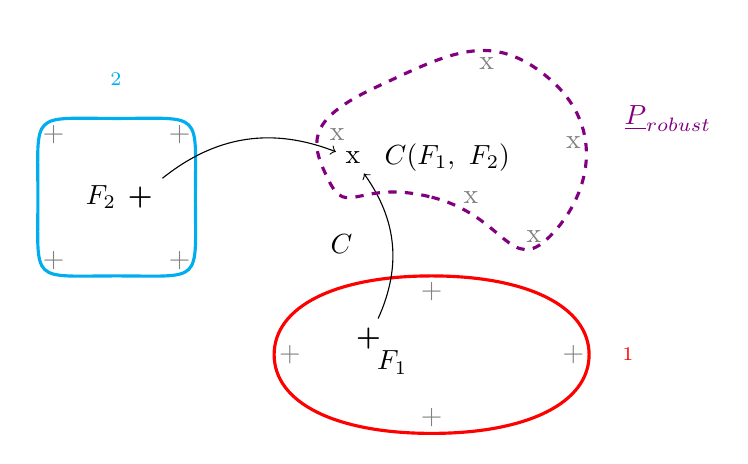
\begin{tikzpicture}[scale=1]
        \draw [red, line width=0.4mm] plot [smooth cycle, tension=1.1] coordinates {(5,1) (7,2) (5,3) (3,2)};
        \draw [cyan, line width=0.4mm] plot [smooth cycle, tension=2] coordinates {(0,4) (1,3) (2,4) (1,5)};
        
        \draw (7.5, 2) node (Belx) {\color{red}$\Bel_1$};
        \draw (1, 5.5) node (Bely) {\color{cyan}$\Bel_2$};
        
        \draw (4.2, 2.2) node (a) {\textbf{+}};
        \draw (4.5, 1.9) node (A) {$F_1$};
        \draw [gray] (5, 1.2) node (+) {+};
        \draw [gray] (6.8, 2) node (+) {+};
        \draw [gray] (5, 2.8) node (+) {+};
        \draw [gray] (3.2, 2) node (+) {+};
        
        
        \draw (1.3, 4) node (b) {\textbf{+}};
        \draw (0.8, 4) node (B) {$F_2$};
        \draw [gray] (0.2, 3.2) node (+) {+};
        \draw [gray] (0.2, 4.8) node (+) {+};
        \draw [gray] (1.8, 3.2) node (+) {+};
        \draw [gray] (1.8, 4.8) node (+) {+};
        
        \draw (4, 4.5) node (c) {x};
        \draw (5.2, 4.5) node (C) {$C(F_1,~F_2)$};
        \draw[->] (a) to [bend right] node[midway, left, inner sep=0.5cm] {$C$}(c);
        \draw[->] (b) to [bend left] (c);
        
        \draw [gray] (3.8, 4.8) node (c) {x};
        \draw [gray] (6.8, 4.7) node (c) {x};
        \draw [gray] (5.7, 5.7) node (c) {x};
        \draw [gray] (6.3, 3.5) node (c) {x};
        \draw [gray] (5.5, 4) node (c) {x};
        
        \draw [violet, dashed, line width=0.4mm] plot [smooth cycle,tension=1.2] coordinates {(3.7, 4.2) (5, 4) (6.5, 3.5) (6.5, 5.5) (4.3, 5.4)};
        
        \draw (8, 5) node (robust) {\color{violet}{$\underline{P}_{robust}$}};
    \end{tikzpicture}
    \caption{Schematic representation of the lower probability $P_{robust}$ of $\M_{robust}$}\label{fig:schema_m_robust}
\end{figure}

\subsection{Copula Applied to Cumulated Mass Functions}\label{sec:joint_mass}
In this section, we will present another way of creating a joint credal set from multiple marginal ones. Consider the same copula $C$ as before and the same marginal credal sets $\M_i$. Each credal set $\M_i$ is fully determined by a mass distribution function $m_i$, which is strictly positive over its $N_i$ focal sets $a^i_1, \dots, a^i_{N_i}$. As described in \cite{ferson_dependence_2004}, it is possible to use the cumulative mass distribution functions as marginals of the copula to create a joint mass distribution function, granted that there is a complete order defined on the focal sets. Links between copulas and belief functions have been investigated in the continuous case in \cite{schmelzer_joint_2015, schmelzer_multivariate_2019}, the special case of necessity functions in \cite{schmelzer_sklars_2015} and of p-boxes in \cite{schmelzer_random_2023}.

Let suppose, without loss of generality, that the marginal focal sets are numbered according to the order $\preceq_i$: $a^i_1\preceq_ia^i_2\preceq_i\dots\preceq_i a^i_{N_i}$. The idea behind this method is to replace the precise marginal CDFs by cumulative masses, to conserve the philosophy behind Sklar's theorem. We thus first define the joint mass $m_\times$ on the product space of focal sets as follows:

\begin{definition}[Joint Mass]\label{def:joint_mass}
    Let $m_1$, \dots, $m_n$ be mass distribution functions over their respective power sets of $\X_1$, \dots, $\X_n$. Suppose that focal sets in each $\X_i$ are ordered and that $a_{k_i}^i$ is the $k_i$-th focal set of $m_i$ according to the chosen order. We define $m_\times$ as the H-volume of copula $C$ computed over the cumulative marginal masses:
    \begin{eqnarray}\label{eq:joint_mass}
        m_\times(a^1_{k_1}\tdt a^n_{k_n}) = H_{\sum_{k=0}^{k_1-1}m_1(a^1_k), \dots, \sum_{k=0}^{k_n-1}m_n(a^n_k)}^{\sum_{k=0}^{k_1}m_1(a^1_k), \dots, \sum_{k=0}^{k_n}m_n(a^n_k)}
    \end{eqnarray}
    with the convention that $\forall i,\, a^i_0=\emptyset$. It is not \textit{strictly} a focal set but allows to deal with the case $k_i=1$ as $m_i(a^i_0)=0$. For sets that are not of the form $a^1_{k_1}\tdt a^n_{k_n}$, the mass $m_\times$ is null.
\end{definition}

\begin{proposition}
    The function $m_\times$ defined in equation \eqref{eq:joint_mass} is a correctly defined mass distribution function over $\X$. 
\end{proposition}
\begin{proof}
    To be a mass distribution function over $\X$, $m_\times$ must verify the 3 properties of definition \ref{def:mass_distribution_function}.
    
    By construction, it holds that $m_\times(\emptyset)=0$, and the properties of the H-volume impose that $m_\times\in[0,1]$.
    
    There are multiple way of proving that $\sum_{A\subseteq\X}m_\times(A)=1$. A direct proof can be done in the case $n=2$, but the notations become quite heavy for any $n>2$. Instead let us use the interpretation of a copula as a multivariate CDF. This method will be also be used in future proofs.
    
    For all \(i\in\opi 0,\, n\cli\) let $F_i$ be a CDF over $[0,\, N_i]$, with, $F_i(j)=\sum_{k=0}^j m_i(a_k^i)$. By Sklar's theorem, $F=C(F_1,\dots, F_n)$ is a multivariate CDF over $[0,\, N_1]\tdt[0,\, N_n]$. Thus it holds that $F([0,\, N_1]\tdt[0,\, N_n])=1$ and:
    \begin{eqnarray*}
        F([0, N_1]\tdt[0, N_n]) &=& F([0, ~\dots, ~0])+\\
        &&F\left(\bigsqcup_{k_1=0}^{N_1-1}\dots\bigsqcup_{k_n=0}^{N_n-1}\left(]k_1, k_1+1]\tdt]k_n, k_n+1]\right)\right)\\
        &=& 0 + \sum_{k_1=0}^{N_1-1}\dots\sum_{k_n=0}^{N_n-1} F(]k_1, k_1+1]\tdt]k_n, k_n+1])\\
        && \text{(CDF of an union of disjoint elements)}\\
        &=& \sum_{k_1=0}^{N_1-1}\dots\sum_{k_n=0}^{N_n-1} H_{F_1(k_1), \dots, F_n(k_n)}^{F_1(k_1+1), \dots, F_n(k_n+1)}\\
        &=& \sum_{k_1=1}^{N_1}\dots\sum_{k_n=1}^{N_n} H_{\sum_{k=0}^{k_1-1}m_1(a^1_k), \dots, \sum_{k=0}^{k_n}m_n(a^n_k)}^{\sum_{k=0}^{k_1}m_1(a^1_k), \dots, \sum_{k=0}^{k_n}m_n(a^n_k)}\\
        &=& \sum_{(a^1_{k_1}\tdt a^n_{k_n})\subseteq\X}m_\times(a^1_{k_1}\tdt a^n_{k_n})
    \end{eqnarray*}
Therefore it holds that:
\begin{eqnarray}
    \sum_{A\subseteq\X}m_\times(A)=\sum_{(a^1_{k_1}\tdt a^n_{k_n})\subseteq\X}m_\times(a^1_{k_1}\tdt a^n_{k_n})=1
\end{eqnarray}
which proves that $m_\times$ is a mass distribution function.
\end{proof}

Having defined a mass distribution function on the product space $\X$, we thus define the joint credal set $\M_{mass}$ and its belief function $\Bel_\times$ as:
\begin{definition}[Joint Belief Function and its Credal Set]\label{def:cumulative_masses_credal_set}
    Let $m_\times$ be the mass distribution function from definition \ref{def:joint_mass}. We note $\Bel_\times$ its joint belief function over the power set of $\X=\X_1\tdt X_n$, \ie:
    \begin{align}
        \forall A\subseteq\X, \Bel_\times(A)=\sum_{a\subseteq A}m_\times(a)\label{eq:joint_belief}
    \end{align}
    Because $\Bel_\times$ is a belief function, it defines a credal set $\M_{mass}$:
    \begin{eqnarray}
        \M_{mass}(C,\M_i) = \{~P:2^\X\rightarrow [0,1] ~|~ \forall A\subseteq\X, P(A)\geqslant \Bel_\times(A)~\}\label{eq:credal_set_mass}
    \end{eqnarray}
\end{definition}

Figure \ref{fig:schema_credal_masss} presents a schematic of $\Bel_\times$ similarly to what was presented with $\M_{robust}$ in figure \ref{fig:schema_m_robust}. In this case, the copula is applied to the lower envelopes instead of being applied point-wise to every CDF from marginal sets. This can lead to differences between $\M_{robust}$ and $\M_{mass}$.
\begin{figure}
    \centering
    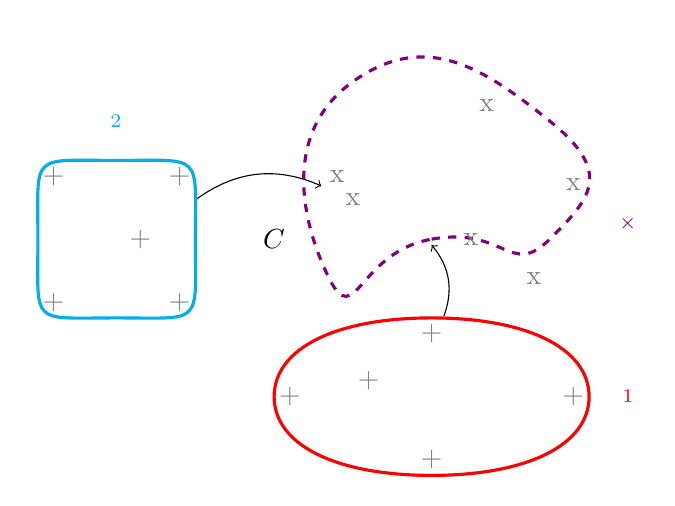
\begin{tikzpicture}[scale=1]
        \draw (7.5, 2) node (Belx) {\color{red}$\Bel_1$};
        \draw (1, 5.5) node (Bely) {\color{cyan}$\Bel_2$};
        
        \draw (5.1, 2.9) node (a) {};
        \draw (5, 4.05) node (b) {};
        \draw (1.88, 4.4) node (c) {};
        \draw (3.6, 4.8) node (d) {};
        
        \draw[->] (a) to [bend right] node[midway, left, inner sep=0.5cm] {} (b.south);
        \draw[->] (c) to [bend left] node[midway, left, inner sep=0.5cm] {} (d.south);
        \draw (3, 4) node (e) {$C$};
        
        \draw [red, line width=0.4mm] plot [smooth cycle, tension=1.1] coordinates {(5,1) (7,2) (5,3) (3,2)};
        \draw [cyan, line width=0.4mm] plot [smooth cycle, tension=2] coordinates {(0,4) (1,3) (2,4) (1,5)};
        \draw [violet, dashed, line width=0.4mm] plot [smooth cycle,tension=1.2] coordinates {(3.7, 3.5) (5, 4) (6.5, 4) (6.5, 5.5) (4, 6) };
        
        \draw (7.5, 4.2) node (mass) {\color{violet}$\Bel_\times$};
        
        \draw [gray] (4.2, 2.2) node (+) {+};
        \draw [gray] (5, 1.2) node (+) {+};
        \draw [gray] (6.8, 2) node (+) {+};
        \draw [gray] (5, 2.8) node (+) {+};
        \draw [gray] (3.2, 2) node (+) {+};
        
        \draw [gray] (1.3, 4) node (+) {+};
        \draw [gray] (0.2, 3.2) node (+) {+};
        \draw [gray] (0.2, 4.8) node (+) {+};
        \draw [gray] (1.8, 3.2) node (+) {+};
        \draw [gray] (1.8, 4.8) node (+) {+};
        
        \draw [gray] (4, 4.5) node (x) {x};
        \draw [gray] (3.8, 4.8) node (x) {x};
        \draw [gray] (6.8, 4.7) node (x) {x};
        \draw [gray] (5.7, 5.7) node (x) {x};
        \draw [gray] (6.3, 3.5) node (x) {x};
        \draw [gray] (5.5, 4) node (x) {x};
    \end{tikzpicture}
    \caption{Schematic representation of the lower probability $\Bel_\times$ of $\M_{mass}$} \label{fig:schema_credal_masss}
\end{figure}

With this way of defining the multivariate mass, the choice of arbitrary orders $\preceq_i$ can have a significant impact on the value of the multivariate mass function. Those order will specifically be ``natural'' orders in sections \ref{subsec:necessity_functions}, \ref{subsec:pboxes} and \ref{subsec:multiple_models}, in the sense where there exists an intuitive total order (inspired by the order on reals). When no natural order exists, the arbitrary choice of the order can greatly impact the output mass or belief functions, as illustrated by the following example.
\todoroman{Quand j'ai $n$ variables j'utilise des notations du style $a_i^n$ (pas trop le choix). Par contre quand j'ai que 2 variables, ça vaudrait peut être le coup de repasser sur des $a_i$ et $b_i$ pour plus de lisibilité ?}
\begin{example}\label{ex:joint_mass}
    Let us present an example in the case $n=2$. Let $m_1$ be a mass distribution function over the power set $2^{\X_1}$ of $\X_1$ with two focal sets $a_1,\, a_2$. Similarly, let $m_2$ be a mass distribution function over the power set $2^\X_2$ with two focal sets $a_1^2,~a_2^2$. Throughout this example we will assume that $a_1^2\preceq_2a_2^2$. We consider the minimum copula $C(u,v)=\min(u,v)$ and that all masses are equal $m_1(a_1^1)=m_1(a_2^1)=m_2(a_1^2)=m_2(a_2^2)=0.5$.
    If there is no natural order on the focal sets of $m_1$, we have to chose an arbitrary one:\par
    $\bullet$ If "$a_1^1\preceq_1a_2^1$" is the arbitrary order (see figure \ref{fig:joint_distrib_arb}), then
    \begin{eqnarray*}
        m_\times(a_1^1,~a_1^2) &=& C(m_1(a_1^1),~m_2(a_1^2))\\
        &=& 0.5\\
        m_\times(a_2^1,~a_1^2) &=& C(1,~m_2(a_1^2)) - C(m_1(a_1^1),~m_2(a_1^2))\\
        &=& m_2(a_1^2) - C(m_1(a_1^1),~m_2(a_1^2))\\
        &=& 0
    \end{eqnarray*}\par
    $\bullet$ If "$a_2^1\preceq_1a_1^1$" is the arbitrary order, then
    \begin{eqnarray*}
        m_\times(a_1^1,~a_1^2) &=& C(1,~m_2(a_1^2)) - C(m_1(a_2^1),~m_2(a_1^2))\\
        &=& m_2(a_1^2) - C(m_1(a_2^1),~m_2(a_1^2))\\
        &=& 0\\
        m_\times(a_2^1,~a_1^2) &=& C(m_1(a_2^1),~m_2(a_1^2))\\
        &=& 0.5
    \end{eqnarray*}
        
    This illustrates that different orders lead to different masses and thus to different credal sets.
    
    \begin{center}
    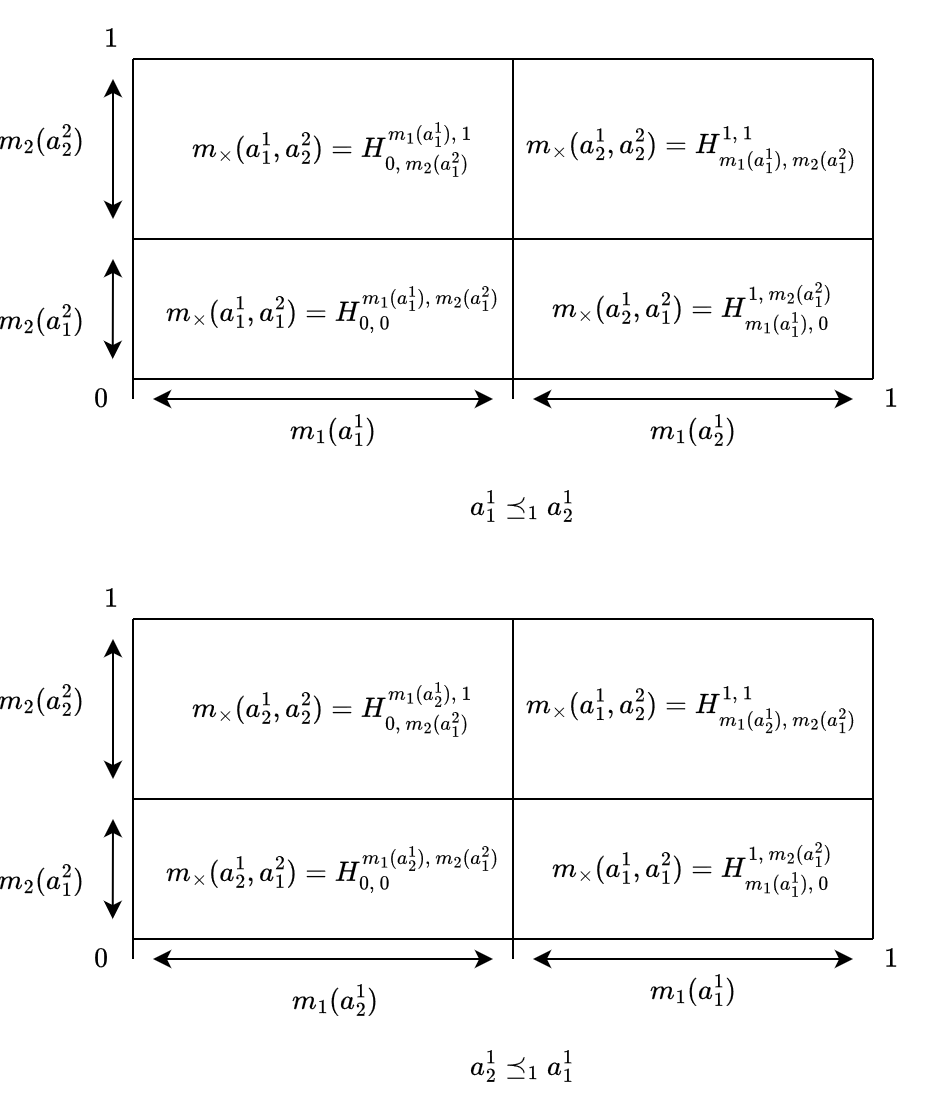
\includegraphics[width=0.8\linewidth]{Images/M_mass_h_volume.png}\captionof{figure}{Joint mass diagram for different orders.}\label{fig:joint_distrib_arb}
    \end{center}
\end{example}

\begin{remark}
    The reason why $\M_{robust}$ is usually different from $\M_{mass}$ is mainly because of the different orders that can exist on focal sets. Consider for instance the minimum copula already presented in example \ref{ex:copulas}:
    \begin{itemize}
        \item In the precise setting, the minimum copula associates the highest probabilities to events with similar values (high-high or low-low), and the lowest probabilities to events with opposite values (low-high).
        \item In the imprecise setting, the concept of high or low values for focal sets does not usually exist. We thus replace it by an order $\preceq$ on focal sets, determining which set is considered ``low'' and which is ``high'' (regardless of the real values actually contained in the set). The minimum copula then associates the highest mass to joint focal sets with similar ``values'' in the sense of the order $\preceq$, and the lowest mass to sets with opposite values in the sense of the order $\preceq$. For instance in the bivariate case, with marginal focal sets $a_1\preceq_1 a_2$ and $b_1\preceq_2 b_2$, using the minimum copula will assign high masses to $a_1\times b_1$ and $a_2\times b_2$ and low masses to $a_1\times b_2$ and $a_2\times b_1$.
    \end{itemize}
    Assigning a high mass to sets containing both low and high values at the same time is something that would not occur in the precise case but is possbile in the imprecise case. This explains the differences between credal sets $\M_{mass}$ and $\M_{robust}$. 
\end{remark}

We saw that $\M_{robust}$ and $\M_{mass}$ can be distinct credal sets. However, because $\M_{robust}$ is difficult to compute, it would be interesting to still use $\M_{mass}$ to approximate it, \ie to verify that $\M_{robust}\subseteq\M_{mass}$ (outer approximation) or $\M_{mass}\subseteq\M_{robust}$ (inner approximation). In example \ref{ex:mass_values}, we show that there is in general no reason for such a relation to exist. Furthermore, if we found an order allowing this relationship, then this order is copula dependent, as changing the copula might break the inclusion. 
\begin{example}\label{ex:mass_values}
    Consider the following setting:
    \begin{itemize}
        \item We consider two spaces $\X_1=\X_2=\{1,~2,~3\}$
        \item We consider two (identical) mass distribution functions $m_1$, $m_2$, each respectively possessing two focal sets $\{2\}$ and $\{1,3\}$.
        \item $m_1(\{2\}) = m_1(\{1,~3\}) = m_2(\{2\})= m_2(\{1,~3\}) = 0.5$
        \item We want to join the credal sets induced by the mass functions using the minimum copula.
    \end{itemize}
    We will compute the bounds of $\M_{mass}$ and $\M_{robust}$ to compare them. The marginals masses being identical and the copula being symmetrical, many results can be obtained by symmetry.
    
    Let us first compute the bounds of $\M_{robust}$. Marginal mass $m_1$ imposes that each marginal probability $P$ will verify:
    \begin{align*}
        \Bel_1(\{2\}) \leqslant &P(\{2\}) \leqslant \Pl_1(\{2\})\\
        0.5 = \sum_{a\subseteq\{2\}}m_1(a) \leqslant &P(\{2\}) \leqslant \sum_{a\cap\{2\}\neq\emptyset}m_1(a) = 0.5
    \end{align*}
    The same result holds for $\{1,~3\}$. We therefore have:
    \begin{align*}
        &P(2)=0.5\\
        &P(1)+P(3)=0.5
    \end{align*}
    And we can compute the same for $m_2$. Looking at those equations, we can deduce that every $P\in\M_{robust}$ verifies:
    \begin{align*}
        0 \leqslant ~&P(\{1\},~ \{1\}) ~\leqslant 0.5\\
        0.5 \leqslant ~&P(\{1, ~2\},~ \{1, ~2\}) ~\leqslant 1
    \end{align*}
    
    Let us now compute the bounds of $\M_{mass}$. Choosing an order between $\{1, ~3\}$ and $\{2\}$ is not intuitive. Suppose that there is a reason which encourages us to chose different orders for the focal sets of $m_1$ and for those of $m_2$, so that $\{1,~3\} \preceq_1 \{2\}$ and $\{2\} \preceq_2 \{1,~3\}$. In this case, it holds that:
    \begin{align*}
        m_\times(\{1, ~3\}, \{2\}) =& ~\min(0.5, ~0.5)\\
        =& ~0.5\\
        m_\times(\{2\}, \{1, ~3\}) =& ~\min(1, ~1) - \min(0.5, ~1)\\
        & - \min(1, ~0.5) + \min(0.5, ~0.5)\\
        =& ~0.5\\
        m_\times(\{2\}, \{2\}) =& ~0\\
        m_\times(\{1, ~3\}, \{1, ~3\}) =& ~0
    \end{align*}
    Thus every probability $P\in\M_{mass}$ will verify:
    \begin{align*}
        0 \leqslant ~&P(\{1\},~ \{1\})~ \leqslant 0\\
        0 \leqslant ~&P(\{1, ~2\},~ \{1, ~2\})~ \leqslant 1
    \end{align*}
    
    Looking at the bounds of $\M_{mass}$ and $\M_{robust}$ on cumulative event $\{1\}\times\{1\}$, we can see that $\M_{robust}\not\subseteq \M_{mass}$. Looking at the bounds on $\{1,2\}\times\{1,2\}$, we can see that $\M_{mass}\not\subseteq \M_{robust}$.
    
    \begin{remark}
        When computing the join mass $m_\times$, we observed that sets $\{2\}\times\{2\}$ and $\{1, 3\}\times\{1, 3\}$ have a null mass, while sets $\{2\}\times\{1, 3\}$ and $\{1, 3\}\times\{2\}$ have a mass of $0.5$. It goes against the expected behaviour of the minimal copula in the precise case, which associates high probabilities to similar values (such as high-high or low-low values). This behaviour stems from the fact that we purposefully chosen different orders $\preceq_1$ and $\preceq_2$ on focal sets, while we cannot reverse the orders on reals in the precise case.
        
        It is legitimate to wonder what would happen if we used the same orders. In that case, it would seem that $\M_{mass}\subset\M_{robust}$. However using the \L ukasiewicz copula, it is possible to keep the same order (where $\{1,~3\} \preceq_1 \{2\}$ and $\{1,~3\} \preceq_2 \{2\}$) while still observing that $\M_{robust}\not\subseteq \M_{mass}$ and $\M_{mass}\not\subseteq \M_{robust}$. Indeed the following bounds for every $P$ in $\M_{robust}$ hold and are reached:
        \begin{align*}
            0 \leqslant ~&P(\{1\}\times\{3\})~ \leqslant 0.5\\
            0 \leqslant ~&P(\{1\}\times\{2\}\cup\{2\}\times\{1\})~ \leqslant 0.5
        \end{align*}
        While $P$ in $\M_{mass}$ verifies:
        \begin{align*}
            0 \leqslant ~&P(\{1\}\times\{3\})~ \leqslant 0\\
            0 \leqslant ~&P(\{1\}\times\{2\}\cup\{2\}\times\{1\})~ \leqslant 1
        \end{align*}
        Finding the values of those bounds follow the same procedure as before but is a much more tedious process, which is thus not detailed here. \comroman{Je n'ai pas inclu les calculs car ils sont un peu longs et fastidieux (il faut expliciter chaque évenement en une somme d'évennements cumulés disjoints, et ensuite simplifier l'expression en utilisant la formulation de la copule). Est-ce que je devrais inclure les calculs en annexe ?}
        
        This means that if we found an order allowing to verify $\M_{robust}\subseteq \M_{mass}$, changing the copula while still keeping the same order might lead to $\M_{robust}\not\subseteq \M_{mass}$.
    \end{remark}
\end{example}

We considered until now that an order has to be chosen arbitrarily. However, special cases of belief functions exhibit a natural order on their focal sets, for instance p-boxes and possibilities. Those special cases will be explored in section \ref{sec:inclusions_between_methods}.

\subsection{Copulas Applied to Belief Functions}\label{sec:aggregation_method}
Another way of joining credal sets with a copula is by directly applying the copula to their lower envelope $\low_i$ for every event:
\begin{definition}[Aggregated Credal Set]\label{def:aggregation_credal_set}
    Given a copula $C$ and $n$ marginal credal sets whose lower probabilities are $\low_1,~\dots,~\low_n$, we define the credal set $\M_{agg}$ over the power set of $\X=\X_1\tdt X_n$ as:
    \begin{eqnarray}
        \M_{agg} = CH(\{P ~|~\forall A_i\subseteq\X_i, P(A_1,\dots, A_n)\geqslant C(\low_1(A_1), \dots, \low_n(A_n)\})\label{eq:copula_on_lower_proba}
    \end{eqnarray}
    where $CH$ is the convex hull from definition \ref{def:convex_hull}.
\end{definition}

Constraints on this set only occur on cylindrical sets of product space $\X_1\tdt \X_n$ (from equation \ref{eq:cylindrical_sets}), contrary to $\M_{mass}$ or $\M_{robust}$, we thus take the convex hull for extending its definition to probabilities on $\X$. We note $\M_{agg}$ this credal set as it uses the copula as an aggregation operator only, without conserving the meaning associated to copulas by Sklar's theorem. In this regard, $\M_{agg}$ has less meaning than $\M_{robust}$ or $\M_{mass}$, but presents the advantage of being easier to compute on cylindrical sets. Figure \ref{fig:meaning_computation} sums up the performances of the different methods in terms of computation cost and meaningfulness.

\begin{figure}[!hb]
    \centering
    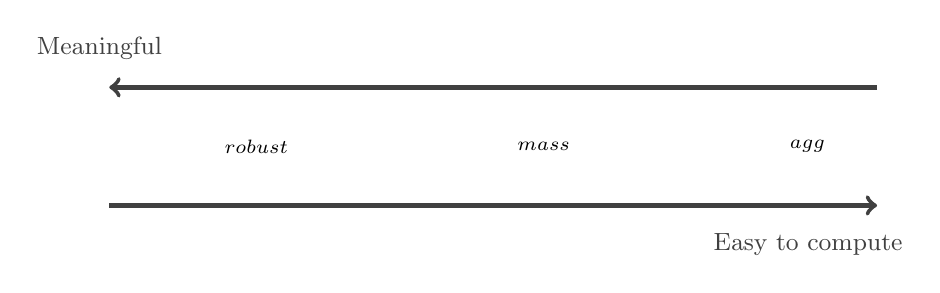
\begin{tikzpicture}[scale=1]
        \draw (0, 0) node (a) {};
        \draw (10, 0) node (b) {};
        \draw (0, 1.5) node (c) {};
        \draw (10, 1.5) node (d) {};
        
        \draw[->, ultra thick, darkgray] (a) to node[midway, left, inner sep=0.5cm] {} (b);
        \draw[->, ultra thick, darkgray] (d) to node[midway, left, inner sep=0.5cm] {} (c);
        
        \draw [darkgray] (9, -0.5) node (z) {\small Easy to compute};
        \draw [darkgray] (0, 2) node (z) {\small Meaningful};
        
        \draw (9, 0.75) node (z) {$\M_{agg}$};
        \draw (5.65, 0.75) node (z) {$\M_{mass}$};
        \draw (2, 0.75) node (z) {$\M_{robust}$};
    \end{tikzpicture}
    \caption{Comparing different methods of joining credal sets with a copula.}
    \label{fig:meaning_computation}
\end{figure}

In general, applying the copula directly to the lower probabilities as in \eqref{eq:copula_on_lower_proba} does not produce a coherent lower probability avoiding sure loss (see definition \ref{def:coherence_sure_loss}). For instance, let us consider $\X_1 = \X_2 = \{1, 2\}$, two lower previsions $\low_1$ and $\low_2$ such that $\low_1(\{1\}) = \low_1(\{2\}) = \low_2(\{1\}) = \low_2(\{2\}) = 0.5$. Joining those two lower probabilities using the minimum copula $C(u,v)=\min(u,v)$ gives a mapping $\low$ which is neither coherent nor avoid sure loss, as presented in Table \ref{tab:non_coherent_lower}.

\begin{table}[!ht]
    \centering
    \begin{tabular}{|c||c|c|}
        \hline
        \hspace{0.2cm} $\low$ \hspace{0.2cm} & \hspace{0.2cm} $\{1\}$ \hspace{0.2cm} & \hspace{0.2cm} $\{2\}$ \hspace{0.2cm} \\\hline\hline
        $\{1\}$ & $0.5$ & $0.5$ \\\hline
        $\{2\}$ & $0.5$ & $0.5$\\
        \hline
        \end{tabular}
        \caption{$\low = \min(\low_1, \low_2)$}
        \label{tab:non_coherent_lower}
\end{table}

\begin{proposition}
    In the special case of the product copula $C_\Pi$, the joint lower probability $\low_{C_\Pi}$ induced by \eqref{eq:copula_on_lower_proba} avoids sure loss if its marginals also avoid sure loss. It follows that for all copulas $C$ dominated by the product copula (\ie $C_\Pi\geqslant C$), and for every $\M_i$ avoiding sure loss, $\M_{agg}(C, \M_i)$ is a non empty credal set.
\end{proposition}

\begin{proof}
    For $i\in\{1,\dots,n\}$, let $\low_i$ be a lower probability avoiding sure lost, \ie whose credal set $\M_i$ contains at least one probability distribution $P_i$. Let us define a multivariate probability $P$ on every $(A_1\tdt A_n)\subseteq\X$ as:
    \begin{eqnarray*}
        P(A_1\tdt A_n) = P_1(A_1)\tdt P_n(A_n)
    \end{eqnarray*}
    Defining $P$ on $(A_1\tdt A_n)\subseteq\X$ is sufficient as those sets contain every atom of $\X$.
    Because $\forall i, P_i\in\M_i,~P_i\geqslant \low_i$, then:
    \begin{eqnarray*}
        P(A_1\tdt A_n) \geqslant \low_1(A_1)\tdt \low_n(A_n) &=& C_\Pi(\low_1(A_1), \dots, \low_n(A_n))\\
        &=& \low_{C_\Pi}(A_1\tdt A_n)
    \end{eqnarray*}
which means $P\in\M_{agg}(C_\Pi, \M_i)$. Therefore $\M_{agg}(C_\Pi, \M_i)$ avoids sure loss if every $\M_i$ avoids sure loss.

Let $C$ be a copula dominated by $C_\Pi$ (\ie $C_\Pi\geqslant C$), and $\low_C$ the lower probability associated with $\M_{agg}(C, \M_i)$. Then it holds that for all $(A_1\tdt A_n)\subseteq\X$:
\begin{eqnarray*}
\low_{C_\Pi}(A_1\tdt A_n)&=&C_\Pi(\low_1(A_1), \dots, \low_n(A_n)) \\
    &\geqslant& C(\low_1(A_1),\dots, \low_n(A_n)) = \low_C(A_1\tdt A_n)
\end{eqnarray*}
which implies that $\M_{agg}(C_\Pi, \M_i)\subseteq \M_{agg}(C, \M_i)$.
\end{proof}

\begin{proposition}
    Conversely, no lower probability $\low_C$ obtained using \eqref{eq:copula_on_lower_proba} with a copula $C$ strictly superior to the product copula by is guaranteed to avoid sure loss. It all depends on the marginal credal sets $\low_i$.
\end{proposition}

\begin{proof}
    Let $C$ be a copula strictly superior to the product. Then there exists $(u_1,\dots,u_n)\in[0,1]^2$ such that:
    \begin{eqnarray*}
        C(u_1,\dots, u_n)~>~u_1\dots u_n
    \end{eqnarray*}
    Let $\M_i$ be marginals credal sets such that $\low_i$ are \textit{precise} probabilities, and that:
    \begin{eqnarray*}
        \forall i,~\exists A_i\in\X_i,~\low_i(A_i)=u_i
    \end{eqnarray*}
    Suppose that $\M_{agg}(C, \M_i)$ avoids sure loss, \ie there is a probability $P$ such that $P\geqslant\low_C$. Let $S$ be a collection of disjoint cylindrical sets of $\X$ (defined in equation \eqref{eq:cylindrical_sets}) covering the complementary event $(A_1\tdt A_n)^c$ of $(A_1\tdt A_n)$. $S$ is defined so that $(A_1\tdt A_n)^c=\bigsqcup_{s\in S}s$.
    Then,
    \begin{eqnarray*}
        P(\X) &=& P\left(\left(A_1\tdt A_n\right)\bigsqcup\left(A_1\tdt A_n\right)^c\right)\\
        &=& P\left(A_1\tdt A_n\right)+P\left((A_1\tdt A_n)^c\right)\\
        &=& P\left(A_1\tdt A_n\right)+\sum_{(s_1\tdt s_n)\in S}P(s_1\tdt s_n)\\
        &\geqslant& \low_C\left(A_1\tdt A_n\right)+\sum_{(s_1\tdt s_n)\in S}\low_C(s_1\tdt s_n)\\
        &>& \low_{C_\Pi}\left(A_1\tdt A_n\right)+\sum_{(s_1\tdt s_n)\in S}\low_{C_\Pi}(s_1\tdt s_n)
    \end{eqnarray*}
    Because we chose $\low_i$ so that they are precise probabilities, their product is also a precise probability. Using the fact that summing probabilities of disjoint events is equal to the probability of their union:
    \begin{eqnarray*}
        \low_{C_\Pi}\left(A_1\tdt A_n\right)+\sum_{(s_1\tdt s_n)\in S}\low_{C_\Pi}(s_1\tdt s_n) &=& \low_{C_\Pi}\left(A_1\tdt A_n\right)+\\
        &&\low_{C_\Pi}\left((A_1\tdt A_n)^c\right)\\
        &=& 1
    \end{eqnarray*}
    This means that $P(\X)>1$ which is impossible. Thus $\M_{agg}(C, \M_i)=\emptyset$ and $\M_{agg}(C, \M_i)$ does not avoid sure loss.
\end{proof}

\section{Inclusions Between Joint Credal Sets}\label{sec:inclusions_between_methods}
Section \ref{sec:methods_for_joining_credal_sets} presented three methods for joining marginal credal sets using a copula. In the general case, there is no reason for the three methods to lead to the same multivariate credal sets. However, for some specific cases on the copulas or on the marginal credal sets, it is possible to find inclusion relationships between the methods. This section explores some of those specific cases. 

\subsection{Using the Product Copula}\label{subsection:product_copula}
In this section, we will consider the case of the product copula $C_\Pi$, representing independence between variables. Using this copula in the robust approach defined by equation \eqref{eq:robust_set} is referred as the strong product in \cite{kacprzyk_factorisation_2010}. Let us denote $\low_{robust}$ the infimum of $\M_{robust}(C_\Pi, \M_i)$ and $\mathcal{S}$ the set from which $\M_{robust}$ is computed (eq. \eqref{eq:robust_ancestor}).
For cylindrical sets $(A_1, \dots, A_n)$ of $\X$, it holds that:
\begin{eqnarray*}
    \low_{robust}(A_1\tdt A_n) &=& \inf\{P(A_1\tdt A_n)~|~P\in\mathcal{S}\}\\
    &=&\inf\{\low_1(A_1)\dots\low_n(A_n)~|~P_i\in\M_i\}\\
    &=&\inf\{\low_1(A_1)~|~P_1\in\M_1\}\dots\inf\{\low_n(A_n)~|~P_n\in\M_n\}\\
    &=&\low_1(A_1)\dots\low_n(A_n)
\end{eqnarray*}
We can split the infimum of a product as a product of infima because we consider mappings with positive values. As this is equivalent of applying the copula directly to the marginals, $\M_{robust}$ and $\M_{agg}$ have the same bounds on cylindrical events. On other events, the lower probabilities are defined as the infimum of the credal sets, thus all bounds are the same and it holds that:
\begin{eqnarray}
    \M_{robust}(C_\Pi, \M_i)\subseteq\M_{agg}(C_\Pi, \M_i)
\end{eqnarray}
This result can also be found in \cite{couso_survey_2000}.
\begin{proposition}
    In the case of the product copula $C_\Pi$, the arbitrary orders on the marginal focal sets have no impact on the value of the joint mass $m_\times$ defined in \eqref{eq:joint_mass}. If $a^1_{k_1}, ~\dots, ~a^n_{k_n}$ is a focal set of $m_1, ~\dots, ~m_n$, then $m_\times$ is given by:
    \begin{eqnarray}\label{eq:joint_mass_product}
        m_\times(a^1_{k_1}\tdt a^n_{k_n}) = m_1(a^1_{k_1})\dots m_n(a^n_{k_n})
    \end{eqnarray}
\end{proposition}

\begin{proof}
    Equation \eqref{eq:joint_mass_product} shows that the order on marginal focal sets does not matter in the case of the product copula. We thus show that equation \eqref{eq:joint_mass_product} holds.
    For simplicity and coherence with the notations of equation \eqref{eq:hvolume}, we will note for all $i\in[0,n]$, $u^i=\sum_{k=0}^{k_i-1}m_i(a_k^i)$, $v^i_k=\sum_{k=0}^{k_i}m_i(a_k^i)$. $\Pi_{i=1}^n\{u_i, v_i\}$ will refer to the Cartesian product $\{u_1, v_1\}\times\{u_2, v_2\}\tdt\{u_n, v_n\}$ and we will note $C_\Pi$ and $H$ as the product copula and its H-volume regardless of their number of marginals. Those notations established, it holds that:
    \begin{eqnarray*}
        m_\times(a^1_{k_1}\tdt a^{n}_{k_{n}}) &=& H_{u_1, \dots, u_{n}}^{v_1, \dots, v_{n}}\\
        &=&\sum_{\substack{(w_1, \dots, w_{n})\in\\\Pi_{i=1}^{n}\{u_i, v_i\}}}(-1)^{|\{k~|~w_k=u_k\}|}C_\Pi(w_1, \dots, w_{n})\\
        &=&\sum_{\substack{(w_1, \dots, w_{n-1})\in\\\Pi_{i=1}^{n-1}\{u_i, v_i\}}}(-1)^{|\{k~|~w_k=\sum_{k=0}^{k_i-1}m_i(a^i_k)\}|}(w_1 \dots w_{n-1}v_{n})\\
        && + \sum_{\substack{(w_1, \dots, w_{n-1})\in\\\Pi_{i=1}^{n-1}\{u_i, v_i\}}}(-1)^{|\{k~|~w_k=\sum_{k=0}^{k_i-1}m_i(a^i_k)\}|+1}(w_1 \dots w_{n-1}u_n)\\
        &=& v_{n}H_{u_1, \dots, u_{n-1}}^{v_1, \dots, v_{n-1}} - u_{n}H_{u_1, \dots, u_{n-1}}^{v_1, \dots, v_{n-1}}\\
        &=& m_{n}(a^{n}_{k_{n}})H_{u_1, \dots, u_{n-1}}^{v_1, \dots, v_{n-1}}
    \end{eqnarray*}
    Doing the same procedure for every variable leads to:
    \begin{eqnarray*}
        m_\times(a^1_{k_1}\tdt a^n_{k_n}) = m_1(a^1_{k_1})\dots m_n(a^n_{k_n})
    \end{eqnarray*}
    which concludes the proof.
\end{proof}

The mass $m_\times$ corresponds to the notion of random set independence presented in \cite{dempster_upper_1967, couso_survey_2000}. Let $\Bel_\times$ be the belief function associated to $m_\times$, and $\forall i\in[1,n], \Bel_i$ the mass function associated to $m_i$. Then for cylindrical sets $(A_1, \dots, A_n)$ of $\X$, it holds that:
\begin{eqnarray}
    \Bel_\times(A_1\tdt A_n) &=& \sum_{(a^1\tdt a^n)\subseteq (A_1, \dots, A_n)}m_\times(a^1\tdt a^n)\nonumber\\
    &=& \sum_{(a^1\tdt a^n)\subseteq (A_1, \dots, A_n)}m_1(a_1)\dots m_n(a^n)\nonumber\\
    &=& (\sum_{a^1\subseteq A_1}m_1(a^1))\dots(\sum_{a^n\subseteq A_n}m_n(a^n))\nonumber\\
    &=& \Bel_1(A_1)\dots \Bel_n(A_n)
\end{eqnarray}

This means that in the case of the product copula $C_\Pi$ with marginals being belief functions, $\M_{robust},~\M_{mass}$ and $\M_{agg}$ all coincide on cylindrical sets. Thus,
\begin{eqnarray*}
    \M_{mass}\subseteq\M_{agg}
\end{eqnarray*}

\subsection{Using the Natural Ordering of Necessity Functions}\label{subsec:necessity_functions}
Necessity functions $\Nec$, also called minitive belief functions, are a special type of belief function verify $\Nec(A\cap B) =\min(\Nec(A), \Nec(B))$ for all events $A, B$ in their domain of definition. In the multivariate case, when a belief is only defined on cylindrical sets, then the minitive property becomes:
\begin{eqnarray}
    &&\forall (A_1\tdt A_n)\subseteq\X, (B_1\tdt B_n)\subseteq\X,\nonumber\\
    &&\Nec(A_1\cap B_1,\dots, A_n\cap B_n) = \min_{(S_1,\dots,S_n)\in\Pi_i\{A_i,B_i\}}(\Nec(S_1, \dots, S_n))
\end{eqnarray}
In \cite{schmelzer_joint_2015}, the author showed that in order to describe the relation between a multivariate belief function and its marginals, in the bivariate case, it is necessary to use a family of sub-copulas: one copula for each tuple of increasing family of events. We remind that a sub-copula is a restriction of a copula to a subset of the unit hyper-cube $[0,1]$ as presented in section \ref{sec:copula_def}.

\begin{theorem}[Sklar's Theorem for Belief Functions \cite{schmelzer_joint_2015}]\label{theorem:sklar_belief}
    Let $\Bel :2^{\X_1}\times2^{\X_2}\rightarrow[0,1]$ be a bivariate belief function and let $\Bel_1$ and $\Bel_2$ denote its marginals over $2^{\X_1}$ and $2^{\X_2}$ respectively. Furthermore, let $\mathcal{I}_1$ and $\mathcal{I}_2$ denote increasing families of subsets of $\X_1$ and $\X_2$. Then there exists a unique sub-copula $C^{\mathcal{I}_1,\mathcal{I}_2}$ on  $\Bel_1(\mathcal{I}_1)\times \Bel_2(\mathcal{I}_2)$ such that:
    \begin{eqnarray}
        \Bel (L_1, L_2) = C^{\mathcal{I}_1,\mathcal{I}_2}(\Bel_1(L_1), \Bel_2(L_2))
    \end{eqnarray}
    for all $L_1\in\mathcal{I}_1,L_2\in\mathcal{I}_2$.
\end{theorem}
For the reverse to be true, it is necessary that $\X_1\in\mathcal{I}_1, \X_2\in\mathcal{I}_2$. Example 1 of \cite{schmelzer_joint_2015} illustrate the need of a copula for each increasing family of events.

Necessity functions are completely determined by their focal sets which form an increasing family of events. Thus by applying Sklar's theorem for belief functions (theorem \ref{theorem:sklar_belief}), it holds that joining two necessity functions with a copula $C$ as in \eqref{eq:copula_on_lower_proba} yields a bivariate belief function (which is not necessarily a necessity function):
\begin{equation}
    \Bel = C(\Nec_1, \Nec_2)\label{eq:sklar_on_necessity}
\end{equation}
where $\Nec_1$ and $\Nec_2$ are the marginal necessity functions. The proof of those results where shown in \cite{schmelzer_joint_2015,schmelzer_sklars_2015}. In the following, we will consider that the focal sets $a^i$ of a necessity functions $\Nec_i$ are already ranked using the natural ordering $\preceq_i$:
\begin{eqnarray}
    \forall (k,j)\in[1, N_i]^2,~k\leqslant j ~\Leftrightarrow ~ a^i_k \preceq_i a^i_j ~\Leftrightarrow ~ a^i_k\subseteq a^i_j
\end{eqnarray}

\begin{proposition}\label{prop:sklar_necessity}
    Joining two marginal necessity functions $\Nec_1, \Nec_2$ with a copula $C$ as in \eqref{eq:sklar_on_necessity} or using the bivariate mass function as in \eqref{eq:joint_mass} with the natural inclusion ordering yields the same bivariate belief function.
\end{proposition}

\begin{proof}
    If we denote by $\Bel_\times$ the belief function defined in \eqref{eq:joint_mass} where the ordering is the inclusion ordering $\preceq_i$ for $i\in[1,2]$. For convenience and with respects to the notations of equation \eqref{eq:hvolume}, we note: $u^i_k=\sum_{j=0}^{k}m_i(a_j^i)$ and consider that $a^i_0=\emptyset$.
    For all focal elements $a_k^1$ of $\Nec_1$ and $a^2_j$ of $\Nec_2$, it holds that:
    \begin{eqnarray*}
        \Bel_\times(a^1_k, a^2_j) &=& \sum_{a^1_p\subseteq a_k^1}\sum_{a^2_q\subseteq a_j^2}m_\times(a^1_p, a^2_q) = \sum_{p=1}^k\sum_{q=1}^j m_\times(a^1_p, a^2_q)\\
        &=&\sum_{p=1}^k\sum_{q=1}^j (~C(u^1_p, u^2_q) + C(u^1_{p-1}, u^2_{q-1}) \\
        &&- C(u^1_{p-1}, u^2_{q}) - C(u^1_{p}, u^2_{q-1})~)\\
        &=&\sum_{p=1}^k\sum_{q=1}^jC(u^1_p, u^2_q) + \sum_{p=0}^{k-1}\sum_{q=0}^{j-1}C(u^1_p, u^2_q) \\
        &&- \sum_{p=0}^{k-1}\sum_{q=1}^jC(u^1_p, u^2_q) - \sum_{p=1}^k\sum_{q=0}^{j-1}C(u^1_p, u^2_q)\\
        &=& C(u^1_k, u^2_j) = C\left(\Nec_1(a_k^1), \Nec_2(a_j^2)\right)\\
    \end{eqnarray*}
    This is the case for necessity function but not in general where:
    \begin{align*}
        \sum_{a^1_p\subseteq a_k^1}\sum_{a^2_q\subseteq a_j^2}m_\times(a^1_p, a^2_q) \neq \sum_{p=1}^k\sum_{q=1}^j m_\times(a^1_p, a^2_q)
    \end{align*}
\end{proof}

Proposition (\ref{prop:sklar_necessity}) considers two marginals. However, it still holds for $n$ marginals, not covered in \cite{schmelzer_sklars_2015}.
\begin{proposition}
   Joining $n$ marginal necessity functions $\Nec_1,~\dots,~\Nec_n$ with a n-copula $C$ as in \eqref{eq:sklar_on_necessity} or using the multivariate variate mass function as in \eqref{eq:joint_mass} with the natural inclusion ordering yields the same multivariate belief function. In other words, for every cylindrical set $(A_1, \dots, A_n)\subseteq\X$, it holds that:
\begin{eqnarray}
    \Bel_\times(A_1\tdt A_n) = C\left(\Nec_1(A_1), \dots, \Nec_n(A_n)\right)
\end{eqnarray}
\end{proposition}

\begin{proof}
    The proof is similar to the one of equation \eqref{eq:joint_mass}, but this time computing the mass of $(a_{k_1}^1\tdt a_{k_n}^n)$ using $F([0,k_1]\tdt[0,k_n])$ and noticing that \begin{eqnarray*}
        \sum_{(a^1_{p_1}\tdt a^n_{p_n})\subseteq(a^1_{k_1}\tdt a^n_{k_n})}m_\times(a^1_{p_1}\tdt a^n_{p_n})=\sum_{p_1=1}^{k_1}\dots\sum_{p_n=1}^{k_n} m_\times(a^1_{p_1}\tdt a^n_{p_n})
    \end{eqnarray*} because all marginals are necessity functions, and the natural inclusion ordered is used for ranking their focal sets.
\end{proof}

\begin{proposition}
    Let $m_\times$ be a joint mass obtained using \eqref{eq:joint_mass}. If $m_\times$ verifies
    \begin{align*}
        \sum_{a^1_p\subseteq a_k^1}\sum_{a^2_q\subseteq a_j^2}m_\times(a^1_p, a^2_q) = \sum_{p=1}^k\sum_{q=1}^j m_\times(a^1_p, a^2_q)
    \end{align*}
    for all marginal focal sets $(a^1_k)$ ,$(a^2_j)$ then its marginals masses correspond to necessity functions. The reverse implication is immediate if we use the natural inclusion order.
\end{proposition}
\begin{proof}
    Let $m_\times$ be a joint mass obtained using \eqref{eq:joint_mass}, with marginal focal sets $(a^1_k)_{1\leqslant k\leqslant N_1}$, $(a^2_j)_{1\leqslant j\leqslant N_2}$ and marginal masses $m_1,m_2$. 
    Let $\Bel_\times$ be its associated belief function verifying
    \begin{align*}
        \sum_{a^1_p\subseteq a^1_k}\sum_{a^2_q\subseteq a_j^2}m_\times(a^1_p, a^2_q) = \sum_{p=1}^k\sum_{q=1}^j m_\times(a^1_p, a^2_q)
    \end{align*}
    for all marginal focal sets $a^1_k,a^2_j$. It is easy to check that
    \begin{align*}
        \sum_{a^2_q\subseteq \X_2}m_\times(a^1_p, a^2_q)=m_1(a^1_p)=\sum_{q=1}^{N_2}m_\times(a^1_p, a^2_q)    
    \end{align*}
    (as we sum the H-volume over a complete partition of $[0,1]$). Thus it holds that:
    \begin{align*}
        \sum_{p=1}^k m_1(a^1_p) = \Bel_\times(a^1_k,\X_2)=\sum_{a^1_p\subseteq a_k^1}m_1(a^1_p)
    \end{align*}
    This result is not sufficient to prove the inclusion of focal sets (there could be a set $a^1_p\subseteq a^1_k,~p>k$ with the same mass value than another set $a^1_{p'}\not\subseteq a^1_k,~p' < k$). Let us show by induction that for all $(k, p)\in\opi1,N_1\cli^2$, $a_1\subset\dots\subset a_k$ and $a_p\not\subseteq a_k$ if $p>k$.
    For the case $k=1$, it holds that:
    \begin{align*}
        \sum_{p=1}^1m_1(a^1_p) &= \sum_{a_p\subseteq a_1}m_1(a^1_p)\\
        \Leftrightarrow m_1(a^1_1) &= m_1(a^1_1) + \sum_{a^1_p\subset a^1_1}m_1(a^1_p)\\
        \Leftrightarrow 0 &=\sum_{a_p\subset a_1}m_1(a^1_p)
    \end{align*}
    which means that no focal set is a strict subset of $a_1$.
    Suppose that there is $k\in\opi1,N_1\cli$ such that: $a_1\subset\dots\subset a_k$ and $\forall p>k,~a_p\not\subseteq a_k$. In particular, $a_{k+1}\not\subseteq a_k$. It holds that:
    \begin{align*}
        \sum_{p=1}^{k+1}m_1(a^1_p) &= \sum_{a^1_p\subseteq a^1_{k+1}}m_1(a^1_p)\\
        \Leftrightarrow m_1(a^1_{k+1}) + \sum_{p=1}^{k} m_1(a^1_p) &= \sum_{a^1_p\subseteq a^1_{k+1}}m_1(a^1_p)\\
        \Leftrightarrow m_1(a^1_{k+1}) + \sum_{a^1_p\subseteq a^1_k} m_1(a^1_p) &= \sum_{a^1_p\subseteq a^1_{k+1}}m_1(a^1_p)\\
        \implies m_1(a^1_{k+1}) &= \sum_{\substack{a^1_p\subseteq a^1_{k+1} \\ a^1_p\not\subseteq a^1_k}} m_1(a^1_p)\\
        \implies m_1(a^1_{k+1}) &= m_1(a^1_{k+1}) + \sum_{\substack{a^1_p\subset a^1_{k+1} \\ a^1_p\not\subseteq a^1_k}} m_1(a^1_p)\\
        \Leftrightarrow 0 &= \sum_{\substack{a^1_p\subset a^1_{k+1} \\ a^1_p\not\subseteq a^1_k}} m_1(a^1_p)
    \end{align*}
    Which means that either there is no focal set that is a strict subset of $a^1_{k+1}$, or that they are all included in $a^1_{k}$. The first case is discarded as:
    \begin{align*}
        \sum_{a^1_p\subseteq a^1_{k+1}}m_1(a^1_p) &= \sum_{p=1}^{k+1}m_1(a^1_p)\\
        \Leftrightarrow \sum_{a^1_p\subset a^1_{k+1}}m_1(a^1_p) &= \sum_{p=1}^{k}m_1(a^1_p)>0
    \end{align*}
    thus $a_1\subset\dots\subset a_{k+1}$.
    Finally, it also holds that:
    \begin{align*}
        \sum_{a^1_p\subseteq a^1_{k+1}}m_1(a^1_p) &= \sum_{p=1}^{k+1}m_1(a^1_p)\\
        \implies \sum_{\substack{a^1_p\subseteq a^1_{k+1} \\ p>k+1}} m_1(a^1_p) + \sum_{\substack{a^1_p\subseteq a^1_{k+1} \\ p\leqslant k+1}} m_1(a^1_p) &= \sum_{p=1}^{k+1}m_1(a^1_p)\\
        \Leftrightarrow \sum_{\substack{a^1_p\subseteq a^1_{k+1} \\ p>k+1}} m_1(a^1_p) &= 0\\
    \end{align*}
    meaning that for all $p>k+1$, $a^1_p\not\subseteq a^1_{k+1}$ which ends the proof by induction. Because all focal sets form a nested family of sets, $\Bel_1$ is a necessity function. The proof for $\Bel $ is identical. 
\end{proof}

As the lower probabilities of $\M_{agg}$ and $\M_{mass}$ coincide on cylindrical sets, the following set equality holds for credal sets $\M_i$ whose lower probabilities are necessity functions:
\begin{eqnarray}\label{eq:inclusion_necessity}
    \M_{mass}(C, \M_i) \subseteq \M_{agg}(C, \M_i)
\end{eqnarray}

Without further assumptions, there is no inclusion relations between $\M_{robust}$ and $\M_{agg}$ or $\M_{mass}$. The following examples present cases where $\inf\M_{robust}<\inf\M_{agg}$ or $\inf\M_{mass}<\inf\M_{robust}$, proving that it is not always possible to get an (inner or outer) approximation of $\M_{robust}$ using $\M_{mass}$ or $\M_{agg}$.

\begin{example}\label{ex:necessity}
    Let $n=2$. Consider $\X_1=\{x^1_1, x^1_2\}$ and $\X_2=\{x^2_1, x^2_2\}$. Let us define two possibility distribution $\pi_1$ and $\pi_2$ over $\X_1$ and $\X_2$ respectively, such that:

    \begin{eqnarray*}
    \begin{cases}
        \pi_1(x^1_1) = 0.1\\
        \pi_1(x^1_2) = 1
    \end{cases}
    \qquad\text{ and }\qquad
    \begin{cases}
        \pi_2(x^2_1)=1\\
        \pi_2(x^2_2)=0.1
    \end{cases}
    \end{eqnarray*}
    
    For $i\in\{1,2\}$, $\pi_i$ generates a necessity measure $\Nec_i$, a possibility measure $\Pi_i$ and a credal set $\M_i$. Let $P_1$ and $P_2$ be two probabilities respectively included in $\M_1$ and $\M_2$,  whose values are indicated in Table \ref{tab:proba_distrib_1}. 
    
    \begin{center}
    \begin{tabular}{|c|c|c|}
        \hline
        $\X_1$ & $x^1_1$ & $x^1_2$\\
        \hline\hline
        $\Nec_1$ & 0 & 0.9\\
        \hline
        $P_1$  & 0.1 & 0.9\\
        \hline
        $\Pi_1$ & 0.1 & 1\\
        \hline
    \end{tabular}
    \quad
    \begin{tabular}{|c|c|c|}
        \hline
        $\X_2$ & $x^2_1$ & $x^2_2$\\
        \hline\hline
        $\Nec_2$ & 0.9 & 0\\
        \hline
        $P_2$  & 0.9 & 0.1\\
        \hline
        $\Pi_2$ & 1 & 0.1\\
        \hline
    \end{tabular}
    \captionof{table}{Probability distributions over $\X_1$ and $\X_2$}
    \label{tab:proba_distrib_1}
    \end{center}

    
    We first consider here the Minimum copula $C_M(u,v)=\min(u,v)$. After joining $P_1$ and $P_2$ with $C_M$ to obtain a joint probability $P_\times$, let us compare its value with the value of the bivariate necessity function $C_M(\Nec_1, \Nec_2)$ on the same event $\{x_2\}\times\{y_1\}$.
    \begin{eqnarray*}
        \Bel_\times(\{x^1_2\}\times\{x^2_1\}) &=& C_M\left(\Nec_1(\{x^1_2\}), \Nec_2(\{x^2_1\})\right)\\
        &=& \min(0.9,~0.9) = 0.9\\
        P_\times(\{x^1_2\}\times\{x^2_1\}) &=& C_M(P_1(\X_1), P_2(\{x^2_1\})) - C_M(P_1(\{x^1_1\}),P_2(x^2_1))\\
        &=& \min(1,~0.9) - \min(0.1,~0.9) = 0.8
    \end{eqnarray*}
    
    We have $P_\times\in\M_{robust}, ~P_\times\not\in\M_{mass}$, which proves that ${M}_{robust}\not\subseteq\M_{mass}$.
    
    Let us now compare the lower bound of $\underline{P}$ of $\M_{robust}$ with that of $\M_{agg}$ but considering the \L ukasiewicz copula $C_L(u,v)=\max(u+v-1,0)$:
    \begin{eqnarray*}
        \Bel_\times(\{x^1_2\}\times\{x^2_1\}) &=& C_L(\Nec_1(\{x^1_2\}), \Nec_2(\{x^2_1\}))\\
        &=& \max(0,~0.9 + 0.9 - 1) = 0.8\\
        \low(\{x^1_2\}\times\{x^2_1\}) &=& \inf_{P_1\in\M_1, P_2\in\M_2}\{C_L(P_1(\{\X_1\}),~P_2(\{x^2_1\})) - C_L(P_1(\{x^1_1\}),\\
        && P_2(\{x^2_1\}))\}\\
        &=& \inf_{P_1\in\M_1, P_2\in\M_2}\{\max(0,~P_1(\X_1) + P_2(\{x^2_1\}) - 1)\\
        && - \max(0,~P_1(\{x^1_1\}) + P_2(\{x^2_1\}) -1)\}\\
        &=& \inf_{P_1\in\M_1, P_2\in\M_2}\{P_2(\{x^2_1\}) - \max(0,~P_1(\{x^1_1\}) + P_2(\{x^2_1\}) - 1 )\}\\
        &=& \inf_{P_1\in\M_1, P_2\in\M_2}\max(P_2(\{x^2_1\}),\\
        && P_2(\{x^2_1\})-P_1(\{x^1_1\}) - P_2(\{x^2_1\}) + 1 )\\
        &\geqslant& \min(\inf_{P_2\in\M_2}\{P_2(\{x^2_1\})\},~\inf_{P_1\in\M_1}\{1-P_1(\{x^1_1\})\}) = 0.9
    \end{eqnarray*}
    
    On this event $\low>Nel_\times$ and because the belief function is coherent then $\M_{mass}\not\subseteq\M_{robust}$ and $\M_{agg}\not\subseteq\M_{robust}$.
\end{example}

\subsection{Using the Natural Ordering of P-boxes}\label{subsec:pboxes}
P-boxes are special cases of belief functions that resemble the most classical CDFs. They are defined with two CDF $\underline{F},~\overline{F}$ such that $\underline{F}\leqslant\overline{F}$, their focal sets $a_\alpha$ are of the form $a_\alpha=[\overline{F}^{-1}(\alpha), \underline{F}^{-1}(\alpha)]$ with $\alpha\in[0,1]$ \cite{destercke_unifying_2008}, where $F^{-1}$ is the inverse of a CDF (or pseudo-inverse if not properly defined). It it thus possible to define a natural order on the focal sets. Let $a_\alpha$ and $a_\beta$ be two focal sets of a p-box $[\underline{F},~\overline{F}]$, with $(\alpha,\beta)\in[0,1]^2$. The natural order $\preceq$ on the focal sets is defined as follows:
\begin{align}
    a_\alpha\preceq a_\beta ~\Leftrightarrow~ \overline{F}^{-1}(\alpha)\leqslant\overline{F}^{-1}(\beta) \text{ and } \underline{F}^{-1}(\alpha)\leqslant\underline{F}^{-1}(\beta)~\Leftrightarrow~ \alpha\leqslant\beta\label{eq:order_pbox}
\end{align}

As it is the case for necessity functions, it is possible to find cases where the sets $\M_{robust}\not\subseteq \M_{mass}$ or $\M_{agg}\not\subseteq\M_{mass}$.
\begin{example}\label{ex:pbox}
    Consider the following p-boxes:
    \begin{center}
    \begin{tabular}{|c|c|c|}
        \hline
        $\X_1$ & $x^1_1$ & $x^1_2$\\
        \hline\hline
        $\underline{F}_1$ & 0 & 1\\
        \hline
        $\overline{F}_1$ & 0.1 & 1\\
        \hline
    \end{tabular}
    \qquad
    \begin{tabular}{|c|c|c|}
        \hline
        $\X_2$ & $x^2_1$ & $x^2_2$\\
        \hline\hline
        $\underline{F}_2$ & 0.9 & 1\\
        \hline
        $\overline{F}_2$ & 1 & 1\\
        \hline
    \end{tabular}
    \captionof{table}{P-boxes over $\X_1$ and $\X_2$}\label{tab:example_pbox}
    \end{center}
    The p-boxes from \ref{tab:example_pbox} lead to the same belief functions as in example \ref{ex:necessity}, thus leading to the same conclusions \ie ${M}_{robust}\not\subseteq\M_{mass}$, $\M_{mass}\not\subseteq\M_{robust}$ and $\M_{agg}\not\subseteq\M_{robust}$.
\end{example}

As stated previously, p-boxes are very closely related to CDF which can motivate one to apply Sklar's theorem (Theorem \ref{theorem:sklar}) to the lower CDF and upper CDF respectively. Given $n$ p-boxes $[\underline{F}_1,~\overline{F}_1],~\dots,~[\underline{F}_n,~\overline{F}_n]$ defined over $\X_1,\dots,\X_n$ and a copula $C$, we can define the lower and upper bounds of a $n$ variate CDF as:
\begin{align*}
    \underline{F}_\times&=C(\underline{F}_1,\dots, \underline{F}_n)\\
    \overline{F}_\times&=C(\overline{F}_1,\dots, \overline{F}_n)
\end{align*}
Sklar's theorem states that $\underline{F}_\times$ and $\overline{F}_\times$ are both CDF, which means that $[\underline{F}_\times, \overline{F}_\times]$ is a multivariate p-box \cite{pelessoni_bivariate_2016, montes_sklars_2015} over cylindrical sets, defining a credal set $\M$. Clearly, the bounds of $\M_{robust}$ on cumulative events are the same as those of the credal set $\M$ induced by the multivariate p-box $[C(\underline{F}_1,\dots, \underline{F}_n),~C(\overline{F}_1,\dots, \overline{F}_n)]$.

\begin{proposition}\label{prop:convexity_pbox}
    When joining masses with a copula $C$ using the natural order on p-boxes \eqref{eq:order_pbox}, it holds that:
    \begin{itemize}
        \item if $C$ is D-convex, then $\M_{mass}\subseteq \M_{agg}$.
        \item if $C$ is D-concave then $\M_{agg}\subseteq\M_{mass}$ 
    \end{itemize}
\end{proposition}

\begin{proof}
    Consider $n$ p-boxes $[\underline{F}_1,~\overline{F}_1],~\dots,~[\underline{F}_n,~\overline{F}_n]$, a D-convex copula $C$ and the natural order on focal sets $(a^i_k)_{1\leqslant k \leqslant N_i}$ of each marginal p-box $[\underline{F}_i,~\overline{F}_i]$. We will denote $m_\times$ the joint mass functions obtained using equations \eqref{eq:joint_mass} and $\Bel_\times$ its associated belief function. We will also refer to $\underline{P}$ as the lower probability associated to $\M_{agg}$ from equation \eqref{eq:copula_on_lower_proba}.

    When considering the natural order on focal sets of a p-box \eqref{eq:order_pbox}, it holds that for every focal set $a^i_p$, the set $\{k~|~a^i_k\subseteq a^i_p\}$ is composed of consecutive integers. In the following, we denote by $\underline{p}$ and $\overline{p}$ the lowest and highest indices of the focal sets included in $a^i_p$. This means that $\{a^i_{\underline{p}}, \dots, a^i_{\overline{p}}\}$ is the set of all focal sets included in $a^i_p$. 

    Let $a^1_{p_1},\dots,a^n_{p_n}$ be focal sets of $m_1,\dots,m_n$. We note $u^i_p=\sum_{k=1}^p m_i(a^i_k)$. It then holds that:
    \begin{align*}
        \Bel_\times(a^1_{p_1}, \dots, a^n_{p_n}) &= \sum_{a^1_{k_1}\subseteq a^1_{p_1}}\dots\sum_{a^n_{k_n}\subseteq a^n_{p_n}}m_\times(a^1_{k_1},\dots, a^n_{k_n})\\
        &= \sum_{k_1=\underline{p}_1}^{\overline{p}_1}\dots\sum_{k_n=\underline{p}_n}^{\overline{p}_n}m_\times(a^1_{k_1},\dots, a^n_{k_n})\\
        &= \sum_{k_1=\underline{p}_1}^{\overline{p}_1}\dots\sum_{k_n=\underline{p}_n}^{\overline{p}_n}H_{u^1_{k_1-1},\dots,u^n_{k_n-1}}^{u^1_{k_1},\dots,u^n_{k_n}}
    \end{align*}
    As the H-volume is computed over a partitioning of $[u^1_{\underline{p}_1-1}, u^1_{\overline{p}_1}]\tdt[u^n_{\underline{p}_n-1} , u^n_{\overline{p}_n}]$, it is possible to greatly simplify the sums. The proof is the same as the proof of \eqref{eq:joint_mass} except that the CDF is computed over $[u^1_{\underline{p}_1-1}, u^1_{\overline{p}_1}]\tdt[u^n_{\underline{p}_n-1} , u^n_{\overline{p}_n}]$ and not $[0,1]^n$. This yields:
    \begin{align*}
        \Bel_\times(a^1_{p_1}, \dots, a^n_{p_n}) = H_{u^1_{\underline{p}_1-1},\dots,u^n_{\underline{p}_n-1}}^{u^1_{\overline{p}_1},\dots,u^n_{\overline{p}_n}}
    \end{align*}
    On the other hand, it holds that:
    \begin{align*}
        \underline{P}(a^1_{p_1}, \dots, a^n_{p_n}) &= C(\Bel_1(a^1_{p_1}),\dots,\Bel_n(a^n_{p_n}))\\
        &= C(\sum_{k_1=\underline{p}_1}^{\overline{p}_1} m_1(a^1_{k_1}), \dots, \sum_{k_n=\underline{p}_n}^{\overline{p}_n} m_1(a^n_{k_n}))\\
        &= C(u^1_{\overline{p}_1} - u^1_{\underline{p}_1-1}, \dots, u^n_{\overline{p}_n} - u^n_{\underline{p}_n-1})
    \end{align*}
    Using equation \eqref{eq:convex_diff_hvol} yields:
    \begin{align*}
        \Bel_\times(a^1_{p_1}, \dots, a^n_{p_n}) \geqslant \underline{P}(a^1_{p_1}, \dots, a^n_{p_n})
    \end{align*}
    The inequality is reversed if $C$ is D-concave, which concludes the proof.
\end{proof}

Figure \ref{fig:copula_convex} illustrates the difference between $\Bel_\times$ and $\underline{P}$ in the case $n=2$.

\begin{figure}[!ht]
    \centering
    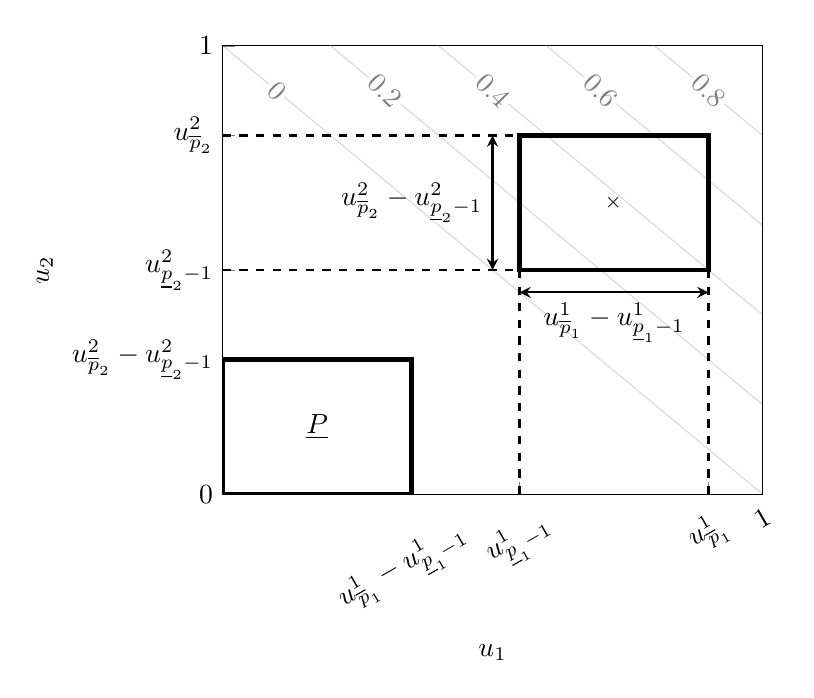
\begin{tikzpicture}
        \begin{axis}[%
            xlabel=$u_1$,
            ylabel=$u_2$,
            xmin=0, xmax=1,
            ymin=0, ymax=1,
            xtick={0.35, 0.55,  0.9, 1},
            xticklabels={$u^1_{\overline{p}_1} - u^1_{\underline{p}_1-1}~~$, $u^1_{\underline{p}_1-1}$, $u^1_{\overline{p}_1}$, $1$},
            ytick={0, 0.3, 0.5,  0.8, 1},
            yticklabels={$0$, $u^2_{\overline{p}_2} - u^2_{\underline{p}_2-1}$, $u^2_{\underline{p}_2-1}$, $u^2_{\overline{p}_2}$, $1$},
            xticklabel style={rotate=30},
            xtick pos=left,
            ytick pos=left,],
            
            \addplot [domain=0:1,samples=40,draw opacity=0.3,color=gray]({x},{1-x});
            \addplot [domain=0:1,samples=40,draw opacity=0.3,color=gray]({x},{1.2-x}); 
            \addplot [domain=0:1,samples=40,draw opacity=0.3,color=gray]({x},{1.4-x}); 
            \addplot [domain=0:1,samples=40,draw opacity=0.3,color=gray]({x},{1.6-x}); 
            \addplot [domain=0:1,samples=40,draw opacity=0.3,color=gray]({x},{1.8-x});

            \node[rotate=-45, fill=white, rounded corners=2pt, inner sep=1pt] (x) at (0.1, 0.9) {\color{gray}0};
            \node[rotate=-45, fill=white, rounded corners=2pt, inner sep=1pt] (x) at (0.3, 0.9) {\color{gray}0.2};
            \node[rotate=-45, fill=white, rounded corners=2pt, inner sep=1pt] (x) at (0.5, 0.9) {\color{gray}0.4};
            \node[rotate=-45, fill=white, rounded corners=2pt, inner sep=1pt] (x) at (0.7, 0.9) {\color{gray}0.6};
            \node[rotate=-45, fill=white, rounded corners=2pt, inner sep=1pt] (x) at (0.9, 0.9) {\color{gray}0.8};
            
            
            \node (a) at (0.9, 0.8) {};
            \node (b) at (0.55, 0.8) {};
            \node (c) at (0.55, 0.5) {};
            \node (d) at (0.9, 0.5) {};
            \draw[ultra thick, black] (c.center) rectangle (a.center) node[pos=0.5]{$\Bel_\times$};
            
            \node (e) at (0, 0.8) {};
            \node (f) at (0, 0.5) {};
            \node (g) at (0.9, 0) {};
            \node (h) at (0.55, 0) {};
            \draw[thick, dashed, black] (e.center) -- (b.center);
            \draw[thick, dashed, black] (f.center) -- (c.center);
            \draw[thick, dashed, black] (g.center) -- (d.center);
            \draw[thick, dashed, black] (h.center) -- (c.center);
            
            \node (i) at (0.35, 0.3) {};
            \node (j) at (0, 0) {};
            \draw[ultra thick, black] (i.center) rectangle (j.center) node[pos=0.5]{$\underline{P}$};
            
            \node (m) at (0.55, 0.45) {};
            \node (n) at (0.9, 0.45) {};
            \node (o) at (0.5, 0.8) {};
            \node (p) at (0.5, 0.5) {};
            \draw [stealth-stealth, thick, black] (m.center) -- (n.center) node[pos=0.5, below]{$u^1_{\overline{p}_1} - u^1_{\underline{p}_1-1}$};
            \draw [stealth-stealth, thick, black] (o.center) -- (p.center) node[pos=0.5, left]{$u^2_{\overline{p}_2} - u^2_{\underline{p}_2-1}$};
        
        \end{axis}
    \end{tikzpicture}
    \caption{Bird view of the \L ukaciewicz 2-copula $C_L$, where the gray lines are the isolines of the copula. $\Bel_\times$ and $\underline{P}$ are represented in the case where the marginals are p-boxes. The thick rectangles represent the bounds on which to compute the H-volume. Numbers $u^i_k$ use the notation of the proof of proposition \ref{prop:convexity_pbox}.}
    \label{fig:copula_convex}
\end{figure}

\subsection{Joining Different Types of Models}\label{subsec:multiple_models}
Different models can be used for multiple sources of uncertainty. When some marginals are modeled using possibility distributions and other by p-boxes, it is still possible to derive results similar as those of sections \ref{subsec:necessity_functions} and \ref{subsec:pboxes} if we use natural orders on the marginal focal sets. 
\begin{proposition}
    When joining marginal credal sets induced by a mix of possibility distributions and p-boxes using a copula $C$ the following inclusion hold:
    \begin{itemize}
        \item if $C$ is D-convex, then $\M_{mass}\subseteq \M_{agg}$.
        \item if $C$ is D-concave then $\M_{agg}\subseteq\M_{mass}$ 
    \end{itemize}
\end{proposition}

\begin{proof}
    The proof is similar to the proof of proposition \ref{prop:convexity_pbox} using the fact that for every focal set $a^i_p$ of a possibility distribution, we can still define $\underline{p}_i$ and $\overline{p}_i$ as $\underline{p}_i=1$ and $\overline{p}_i=p$. The rest of the proof is identical.
\end{proof}

\subsection{Using Other Orders}
Instead of considering the natural ordering, or when such an order does not exists, one could consider an arbitrary order between focal sets when defining $\M_{mass}$ as in \eqref{eq:joint_mass}. A few questions arise: is there always an arbitrary order allowing $\M_{robust}\subseteq\M_{mass}$? If such an order exists, is it possible to explicit it in advance, \ie without computing the lower bounds of the credal sets?

It appears that an order allowing $\M_{robust}\subseteq\M_{mass}$ does not always exist. To prove it, let us find an example where no order allows either inclusion.
\begin{example}
Consider the Clayton copula for $\theta=2$ and $n=2$:
\begin{eqnarray*}
    \forall (u_1,u_2)\in\mathbb{R}^2\backslash(0,0), ~C(u_1,u_2)=\frac{u_1u_2}{\sqrt{{u_1}^2+{u_2}^2-{u_2}^2{u_2}^2}}
\end{eqnarray*}
and $C(0,0)=0$ by continuity (we simplified the expression of the copula given in table \ref{tab:familiy_of_copula}). Let us consider $\X_1=\{x^1_1,\, x^1_2,\, x^1_3\}$, $\X_2=\{x^2_1,\, x^2_2,\, x^2_3\}$ and two possibility distributions $\pi_1$, $\pi_2$ over $\X_1$ and $\X_2$ respectively:
\begin{eqnarray*}
    \pi_1(x^1_1)=\pi_2(x^2_1)=0.2 \qquad \pi_1(x^1_2)=\pi_2(x^2_2)=1 \qquad \pi_1(x^1_3)=\pi_2(x^2_3)=0.7 
\end{eqnarray*}
and the marginal credal sets $\M(\pi_1)$, $\M(\pi_2)$ they induce. We note the focal sets as $a^1_1=\{x^1_2\},~a^1_2=\{x^1_2,\, x^1_3\},~a^1_3=\{x^1_1,\,x^1_2,\,x^1_3\}$ and $a^2_1=\{x^2_2\},~a^2_2=\{x^2_2,\, x^2_3\},~a^2_3=\{x^2_1,\, x^2_2,\, x^2_3\}$. By joining $\M(\pi_1)$ and $\M(\pi_2)$ using $C$, we can obtain the lower probability $\low$ of $\M_{robust}$ using equation \eqref{eq:robust_set}, and a total of 6 belief functions $\Bel^{\preceq_1,\preceq_2}_\times$ using equation \eqref{eq:joint_mass} depending on the orders $\preceq_1, \preceq_2$ used to join the marginal masses. For instance if $\preceq_1$ is such that $a^1_3\preceq_1 a^1_1 \preceq_1 a^1_2$ and $\preceq_2$ such that $a^2_1 \preceq_2 a^2_2 \preceq_2 a^2_3$, then the bivariate mass $m_\times$ would be defined as follows:
\begin{eqnarray*}
    m_\times(a^1_3\times a^2_1) &=& C(m_1(a^1_3), m_2(a^2_1))\\
    m_\times(a^1_1\times a^2_1) &=& C(m_1(a^1_3)+m_1(a^1_1), m_2(a^2_1)) - C(m_1(a^1_3), m_2(a^2_1))\\
    m_\times(a^1_3\times a^2_2) &=& C(m_1(a^1_3), m_2(a^2_1) + m_2(a^2_2)) - C(m_2(a^1_3), m_2(a^2_1))\\
    &\dots&
\end{eqnarray*}

If we consider the two events $E_1=\{x^1_2\}\times\{x^2_2,~x^2_3\}$ and $E_2=\{x^1_2,~x^1_3\}\times\{x^2_2\}$, it is possible to show that $\low(E_1)=\low(E_2)\approx0.131$ (by symmetry of the problem) which is obtained for:
\begin{align*}
    &P_1(x^1_1)=0, \qquad&P_1(x^1_2)=0.3, \qquad&P_1(x^1_3)=0.7,\\
    &P_2(x^2_1)=0.2, \qquad&P_2(x^2_2)=0.3, \qquad&P_2(x^2_3)=0.5
\end{align*}
for $E_1$, and similarly with $P_1$ and $P_2$ reversed for $E_2$. Those values were estimated by running simulations, but their exact value can be computed by solving an optimization problem as $C$ is differentiable (although it is a bit tedious to compute). Then for all orders $\preceq_1,~\preceq_2$ on the focal sets of $\pi_1$ and $\pi_2$ it holds:

 \begin{align*}
    \begin{cases}
        \begin{split}
            \Bel_\times^{\preceq_1,\preceq_2}(E_1) \leqslant& \low(E_1)\\
            \Bel_\times^{\preceq_1,\preceq_2}(E_2) >& \low(E_2)
        \end{split}
    \end{cases}
    \qquad\text{ or }\qquad
    \begin{cases}
        \begin{split}
            \Bel_\times^{\preceq_1,\preceq_2}(E_1) >& \low(E_1)\\
            \Bel_\times^{\preceq_1,\preceq_2}(E_2) \leqslant& \low(E_2)
        \end{split}
    \end{cases}
\end{align*}

The table \ref{tab:beliefs_orders} shows a rounded value of $\Bel^{\preceq_1,\preceq_2}_\times$ for all orders for events $E_1$, $E_2$.

\begin{center}
\begin{tabular}{|c||c|c|c|}
\hline
$\Bel^{\preceq_1,\preceq_2}_\times(\mathbf{E_1})$ & $a^2_3\preceq_2a^2_2\preceq_2a^2_1$ & $a^2_3\preceq_2a^2_1\preceq_2a^2_2$ & $a^2_2\preceq_2a^2_3\preceq_2a^2_1$ \\ \hline\hline
$a^1_3\preceq_1a^1_2\preceq_1a^1_1$ & 0.296 & 0.296 & 0.224 \\ \hline
$a^1_3\preceq_1a^1_1\preceq_1a^1_2$ & 0.254 & 0.254 & 0.240 \\ \hline
$a^1_2\preceq_1a^1_3\preceq_1a^1_1$ & 0.296 & 0.296 & 0.224 \\ \hline
$a^1_1\preceq_1a^1_3\preceq_1a^1_2$ & \textbf{0.131} & \textbf{0.131} & 0.279 \\ \hline
$a^1_2\preceq_1a^1_1\preceq_1a^1_3$ & 0.291 & 0.291 & 0.216 \\ \hline
$a^1_1\preceq_1a^1_2\preceq_1a^1_3$ & \textbf{0.131} & \textbf{0.131} & 0.279 \\ \hline
\end{tabular}

\vspace{0.5cm}

\begin{tabular}{|c||c|c|c|}
\hline
$\Bel^{\preceq_1,\preceq_2}_\times(\mathbf{E_1})$ & $a^2_1\preceq_2a^2_3\preceq_2a^2_2$ & $a^2_2\preceq_2a^2_1\preceq_2a^2_3$ & $a^2_1\preceq_2a^2_2\preceq_2a^2_3$ \\ \hline\hline
$a^1_3\preceq_1a^1_2\preceq_1a^1_1$ & 0.259 & 0.180 & 0.180 \\ \hline
$a^1_3\preceq_1a^1_1\preceq_1a^1_2$ & 0.208 & 0.270 & 0.270 \\ \hline
$a^1_2\preceq_1a^1_3\preceq_1a^1_1$ & 0.259 & 0.180 & 0.180 \\ \hline
$a^1_1\preceq_1a^1_3\preceq_1a^1_2$ & 0.251 & 0.293 & 0.293 \\ \hline
$a^1_2\preceq_1a^1_1\preceq_1a^1_3$ & 0.236 & 0.218 & 0.218 \\ \hline
$a^1_1\preceq_1a^1_2\preceq_1a^1_3$ & 0.251 & 0.293 & 0.293 \\ \hline
\end{tabular}

\vspace{1cm}

\begin{tabular}{|c||c|c|c|}
\hline
$\Bel^{\preceq_1,\preceq_2}_\times(\mathbf{E_2})$ & $a^2_3\preceq_2a^2_2\preceq_2a^2_1$ & $a^2_3\preceq_2a^2_1\preceq_2a^2_2$ & $a^2_2\preceq_2a^2_3\preceq_2a^2_1$ \\ \hline\hline
$a^1_3\preceq_2a^1_2\preceq_2a^1_1$ & 0.296 & 0.254 & 0.296 \\ \hline
$a^1_3\preceq_1a^1_1\preceq_1a^1_2$ & 0.296 & 0.254 & 0.296 \\ \hline
$a^1_2\preceq_1a^1_3\preceq_1a^1_1$ & 0.224 & 0.240 & 0.224 \\ \hline
$a^1_1\preceq_1a^1_3\preceq_1a^1_2$ & 0.259 & 0.208 & 0.259 \\ \hline
$a^1_2\preceq_1a^1_1\preceq_1a^1_3$ & 0.180 & 0.270 & 0.180 \\ \hline
$a^1_1\preceq_1a^1_2\preceq_1a^1_3$ & 0.180 & 0.270 & 0.180 \\ \hline
\end{tabular}

\vspace{0.5cm}

\begin{tabular}{|c||c|c|c|}
\hline
$\Bel^{\preceq_1,\preceq_2}_\times(\mathbf{E_2})$ & $a^2_1\preceq_2a^2_3\preceq_2a^2_2$ & $a^2_2\preceq_2a^2_1\preceq_2a^2_3$ & $a^2_1\preceq_2a^2_2\preceq_2a^2_3$ \\ \hline\hline
$a^1_3\preceq_2a^1_2\preceq_2a^1_1$ & \textbf{0.131} & 0.291 & \textbf{0.131} \\ \hline
$a^1_3\preceq_1a^1_1\preceq_1a^1_2$ & \textbf{0.131} & 0.291 & \textbf{0.131} \\ \hline
$a^1_2\preceq_1a^1_3\preceq_1a^1_1$ & 0.279 & 0.216 & 0.279 \\ \hline
$a^1_1\preceq_1a^1_3\preceq_1a^1_2$ & 0.251 & 0.236 & 0.251 \\ \hline
$a^1_2\preceq_1a^1_1\preceq_1a^1_3$ & 0.293 & 0.218 & 0.293 \\ \hline
$a^1_1\preceq_1a^1_2\preceq_1a^1_3$ & 0.293 & 0.218 & 0.293 \\ \hline
\end{tabular}
\captionof{table}{Value of $\Bel^{\preceq_1,\preceq_2}_\times$ for $E_1$ and $E_2$ depending on the arbitrary orders $\preceq_1$, $\preceq_2$. Values in bald font represent the minimal value attained by the different belief functions, where $\Bel^{\preceq_1,\preceq_2}_\times(E)=\low(E)$.}
\label{tab:beliefs_orders}
\end{center}

Answering the question ``if an order allowing $\M_{robust}\subseteq\M_{mass}$ exists, is it possible to explicit it in advance?'' is not as trivial. Indeed the order will be dependent of the copula. We ran simulations where we created different possibility distributions (for $card(\X_1)=card(\X_2)\in\{3,4\}$), sampled the marginal credal sets and joined them with a copula $C$ to get $\inf\M_{robust}$ and compared its values with the one of $\Bel^{\preceq_1,\preceq_2}$.
\begin{itemize}
	\item When running the simulation with the lower Fréchet–Hoeffding copula $C(u,v)=\max(0,u+v-1)$, we observe that a specific couple of order always works: $\preceq_1:~a^1_3\preceq_1a^1_2\preceq_1a^1_1$ and $\preceq_2~a^2_3\preceq_2a^2_2\preceq_2a^2_1$, while other orders do not permit the inclusion $\M_{robust}\subseteq\M_{mass}$ all the time.
\end{itemize}
The order is thus copula dependent.

We ran simulation for the lower and upper Fréchet-Hoeffding copulas, as well as with the copulas presented in table \ref{tab:familiy_of_copula}. We were only able to find examples where no orders were working for the Ali-Mikail-Haq copula with $\theta>0$, for the Gumbel copula and for Clayton copulas. 
\end{example}
\pagebreak